%%%%%%%%%%%%%%%%%%%%%%% file template.tex %%%%%%%%%%%%%%%%%%%%%%%%%
%
% This is a general template file for the LaTeX package SVJour3
% for Springer journals.          Springer Heidelberg 2010/09/16
%
% Copy it to a new file with a new name and use it as the basis
% for your article. Delete % signs as needed.
%
% This template includes a few options for different layouts and
% content for various journals. Please consult a previous issue of
% your journal as needed.
%
%%%%%%%%%%%%%%%%%%%%%%%%%%%%%%%%%%%%%%%%%%%%%%%%%%%%%%%%%%%%%%%%%%%
%
% First comes an example EPS file -- just ignore it and
% proceed on the \documentclass line
% your LaTeX will extract the file if required
\begin{filecontents*}{example.eps}
%!PS-Adobe-3.0 EPSF-3.0
%%BoundingBox: 19 19 221 221
%%CreationDate: Mon Sep 29 1997
%%Creator: programmed by hand (JK)
%%EndComments
gsave
newpath
  20 20 moveto
  20 220 lineto
  220 220 lineto
  220 20 lineto
closepath
2 setlinewidth
gsave
  .4 setgray fill
grestore
stroke
grestore
\end{filecontents*}
%
\RequirePackage{fix-cm}
%
%\documentclass{svjour3}                     % onecolumn (standard format)
%\documentclass[smallcondensed]{svjour3}     % onecolumn (ditto)
\documentclass[smallextended]{svjour3}       % onecolumn (second format)
%\documentclass[twocolumn]{svjour3}          % twocolumn
%
\smartqed  % flush right qed marks, e.g. at end of proof
%
\usepackage{graphicx}
\usepackage{epstopdf}
%
% \usepackage{mathptmx}      % use Times fonts if available on your TeX system
%
% insert here the call for the packages your document requires
%\usepackage{latexsym}
% etc.
%
% please place your own definitions here and don't use \def but
% \newcommand{}{}
%
% Insert the name of "your journal" with
% \journalname{myjournal}
%
\begin{document}


\title{Multi-modality Imagery Database for Plant Phenotyping %\thanks{Grants or other notes
%about the article that should go on the front page should be
%placed here. General acknowledgments should be placed at the end of the article.}
}
%\subtitle{Do you have a subtitle?\\ If so, write it here}

%\titlerunning{Short form of title}        % if too long for running head

\author{First Author         \and
        Second Author %etc.
}

%\authorrunning{Short form of author list} % if too long for running head

\institute{F. Author \at
              first address \\
              Tel.: +123-45-678910\\
              Fax: +123-45-678910\\
              \email{fauthor@example.com}           %  \\
%             \emph{Present address:} of F. Author  %  if needed
           \and
           S. Author \at
              second address
}

\date{Received: date / Accepted: date}
% The correct dates will be entered by the editor


\maketitle

\begin{abstract}
Insert your abstract here. Include keywords, PACS and mathematical
subject classification numbers as needed.
\keywords{Plant Phenotyping  \and Computer Vision \and Plant image \and Leaf segmentation \and Leaf tracking\and Multiple sensors \and Arabidopsis \and Bean}
% \PACS{PACS code1 \and PACS code2 \and more}
% \subclass{MSC code1 \and MSC code2 \and more}
\end{abstract}

\section{Introduction}
\label{sec:intro}

With the rapid growth of world population and the loss of arable land, there is an increasing desire to improve the yield and quality of crops.  Key to increasing yields is gaining understanding of the genetic mechanisms that influence plant growth~\cite{doos2002population}.
%
A classic genetic approach is to produce a diverse population of mutant lines, grow them either in growth chambers with simulated environmental conditions or directly in the field, visually observe the plants during the growth period, and finally identify plant morphological or physiological patterns that tightly associate with key growth factors~\cite{houle2010phenomics}.
%
While many factors can be assessed quantitatively, which is essential for high-throughput study, one of the bottleneck in this research pipeline is plant visual phenotyping~\cite{walter2015plant}.

\begin{figure*}
\begin{centering}
\begin{tabular}{@{}c c c c c}
%\begin{tabular}{lllllllll}
(a) &
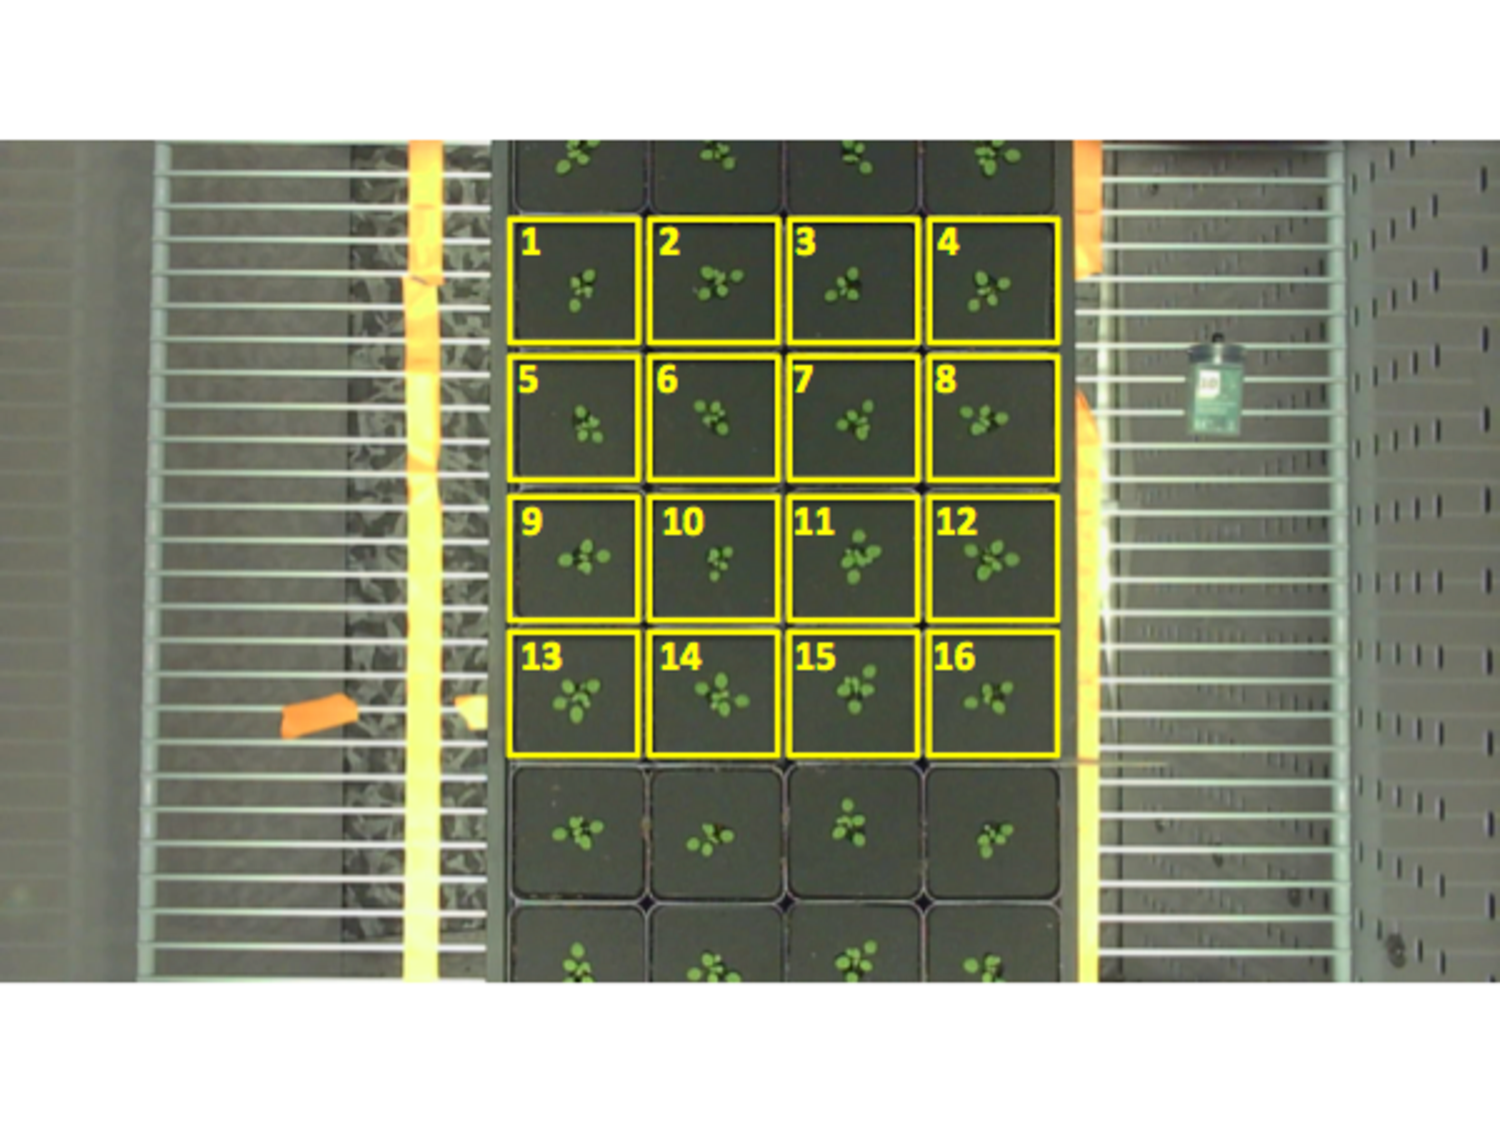
\includegraphics[width=.23\textwidth]{Figures/FourModalities/A_rgb}&
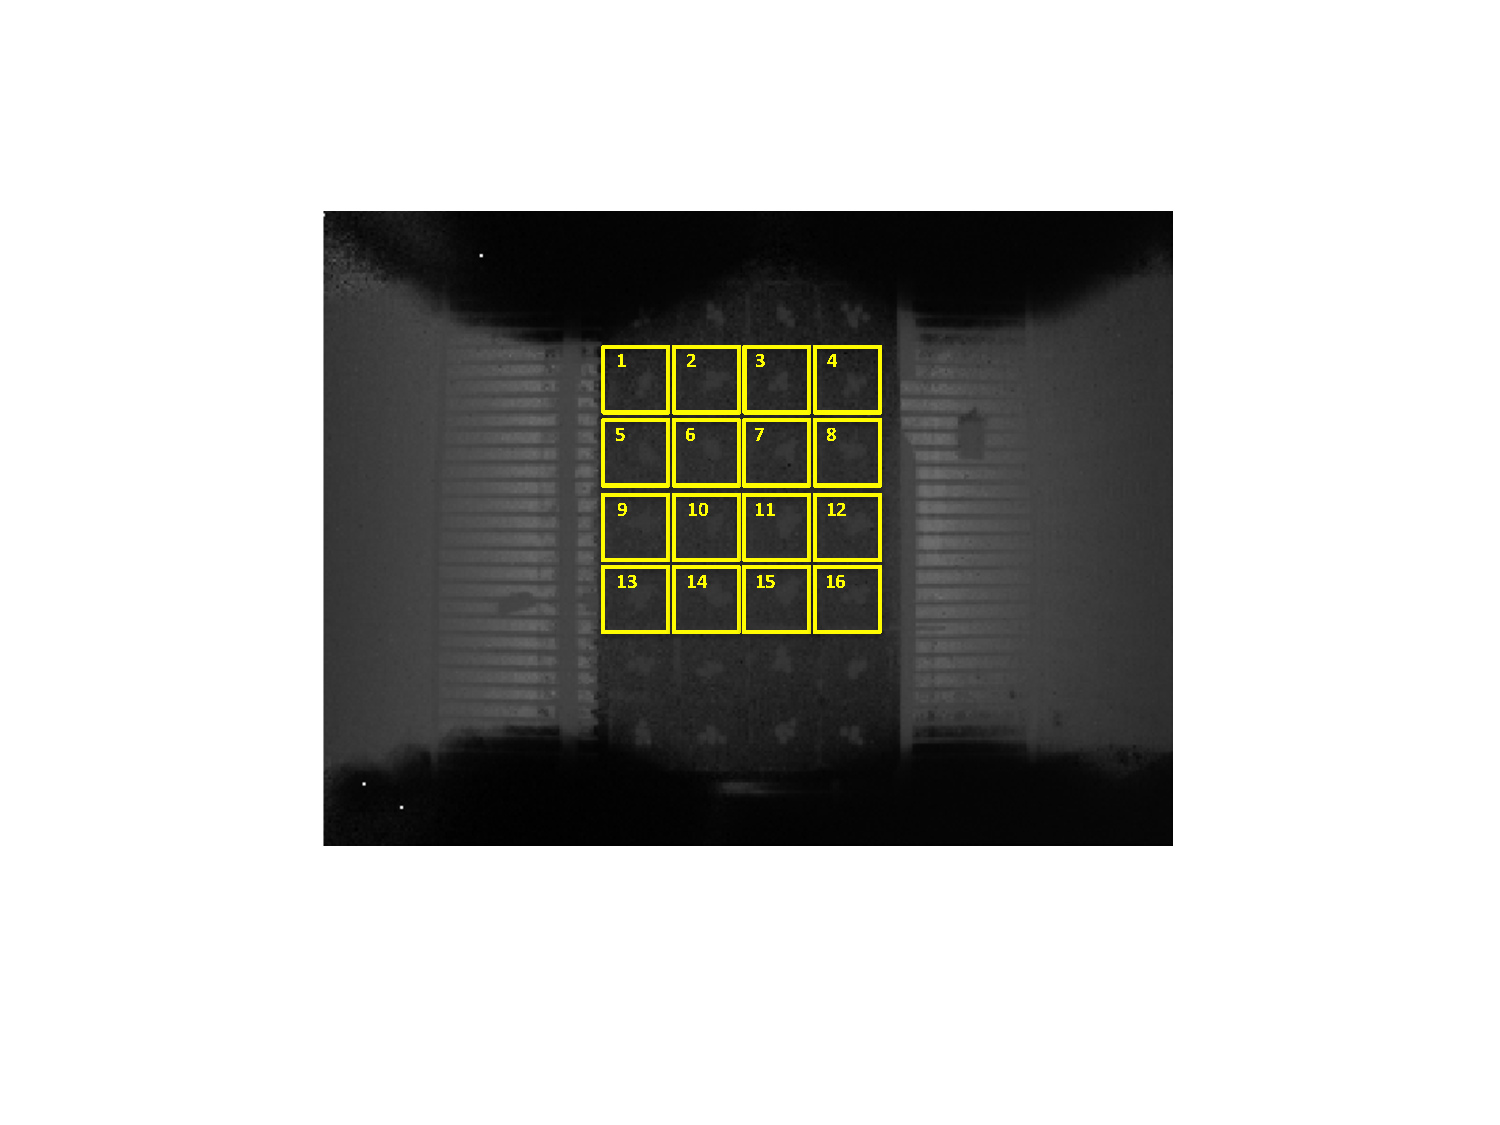
\includegraphics[width=.23\textwidth]{Figures/FourModalities/A_depth}&
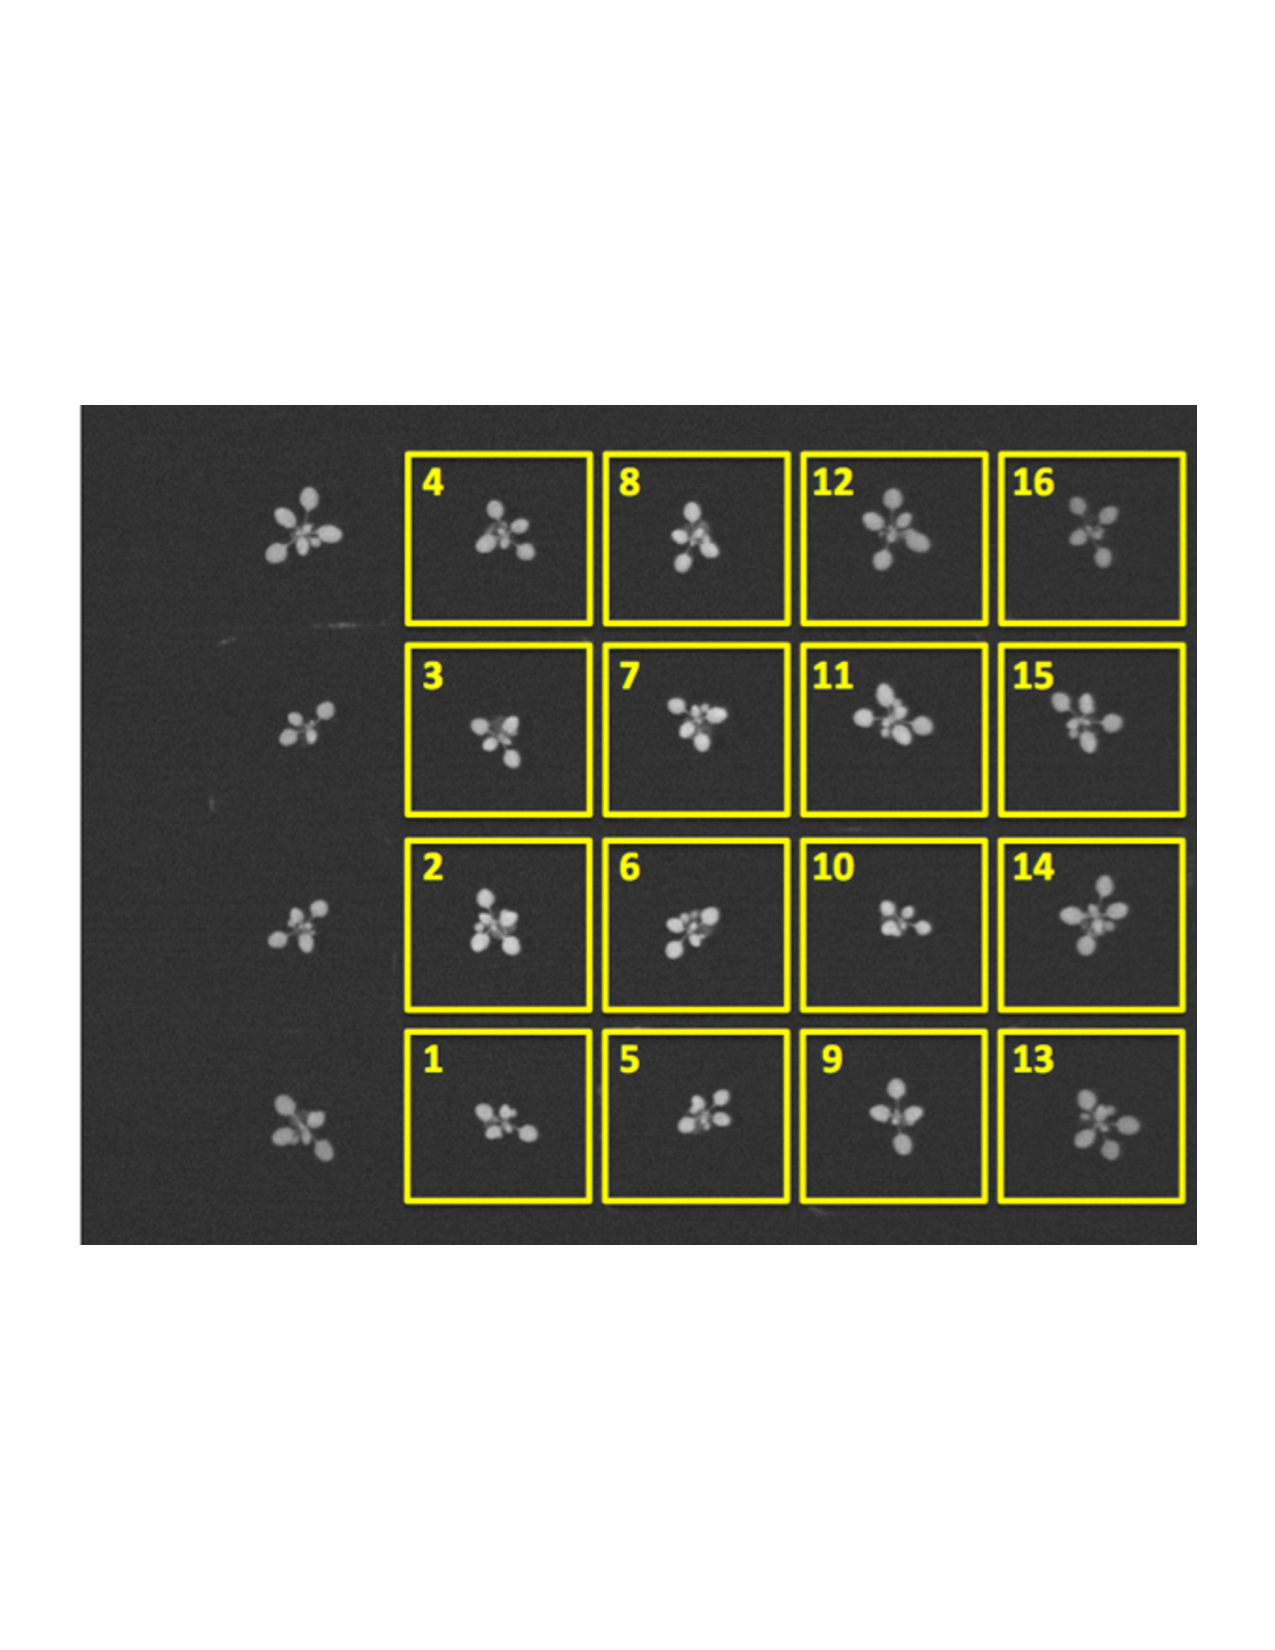
\includegraphics[width=.23\textwidth]{Figures/FourModalities/A_fmp}&
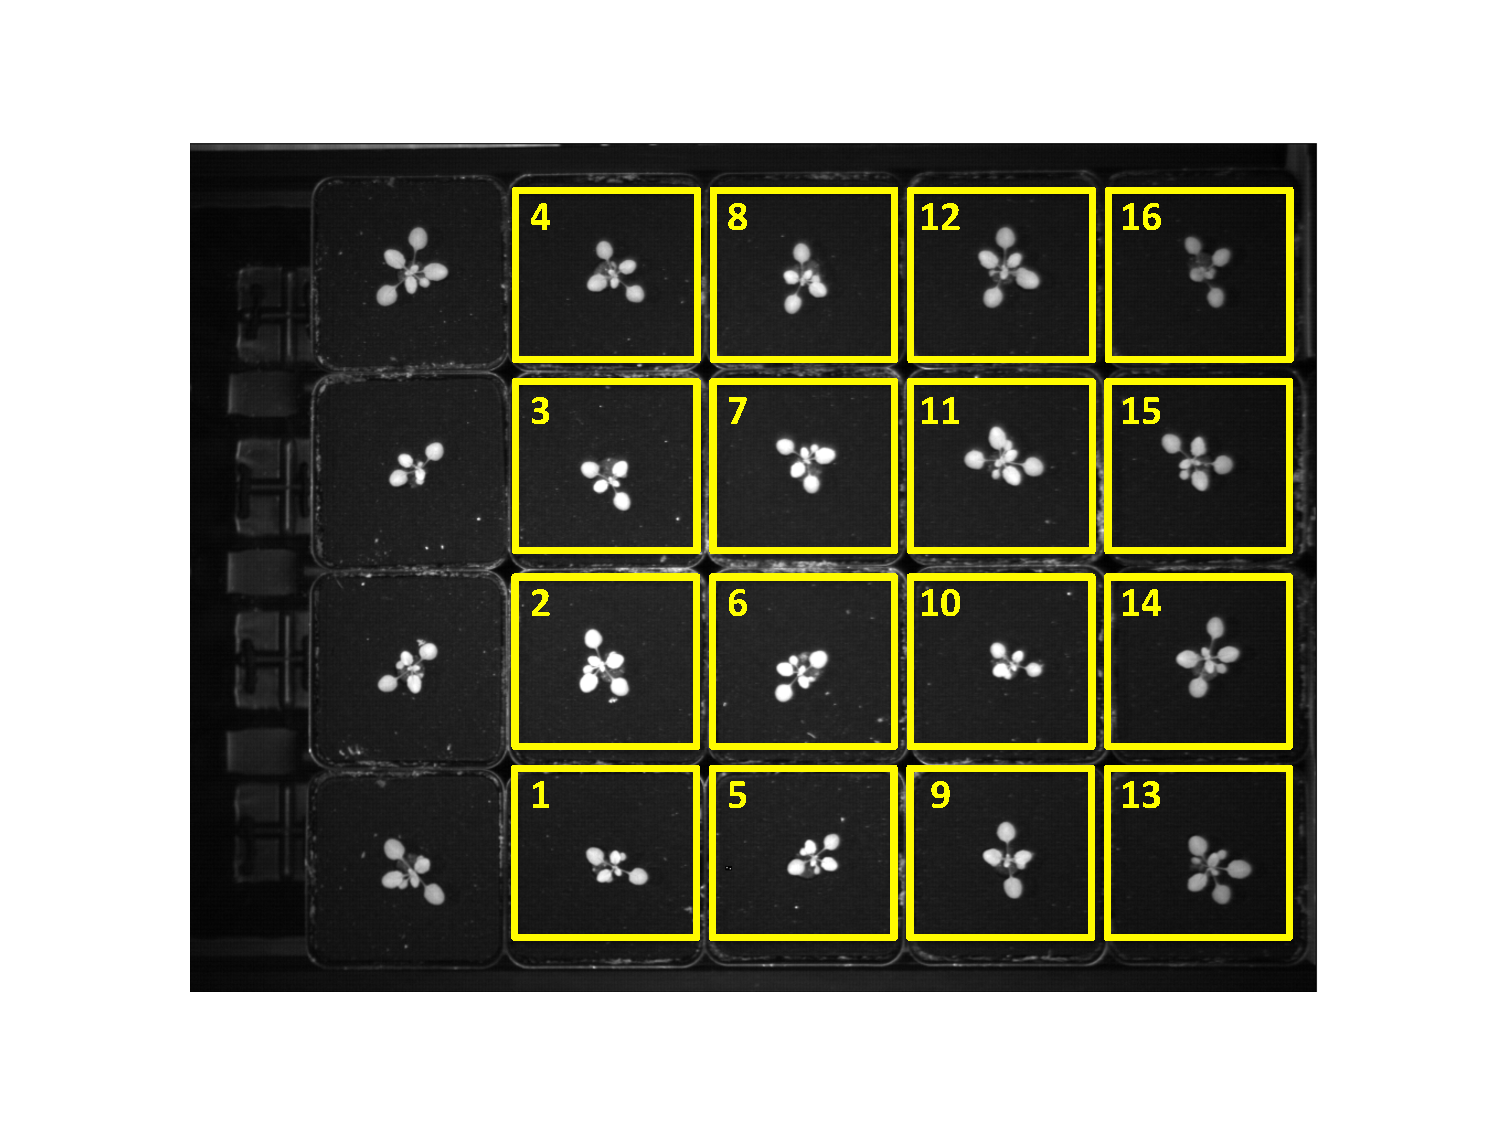
\includegraphics[width=.23\textwidth]{Figures/FourModalities/A_ir}\\
(b) &
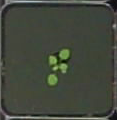
\includegraphics[width=.1\textwidth]{Figures/FourModalities/A1_rgb}&
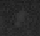
\includegraphics[width=.1\textwidth]{Figures/FourModalities/A1_depth}&
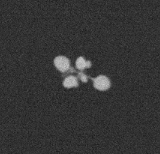
\includegraphics[width=.1\textwidth]{Figures/FourModalities/A1_fmp}&
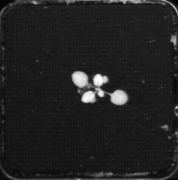
\includegraphics[width=.1\textwidth]{Figures/FourModalities/A1_ir}\\
%Arabidopsis: RGB & Arabidopsis: depth & Arabidopsis: fluorescence & Arabidopsis: IR \\
(c) &
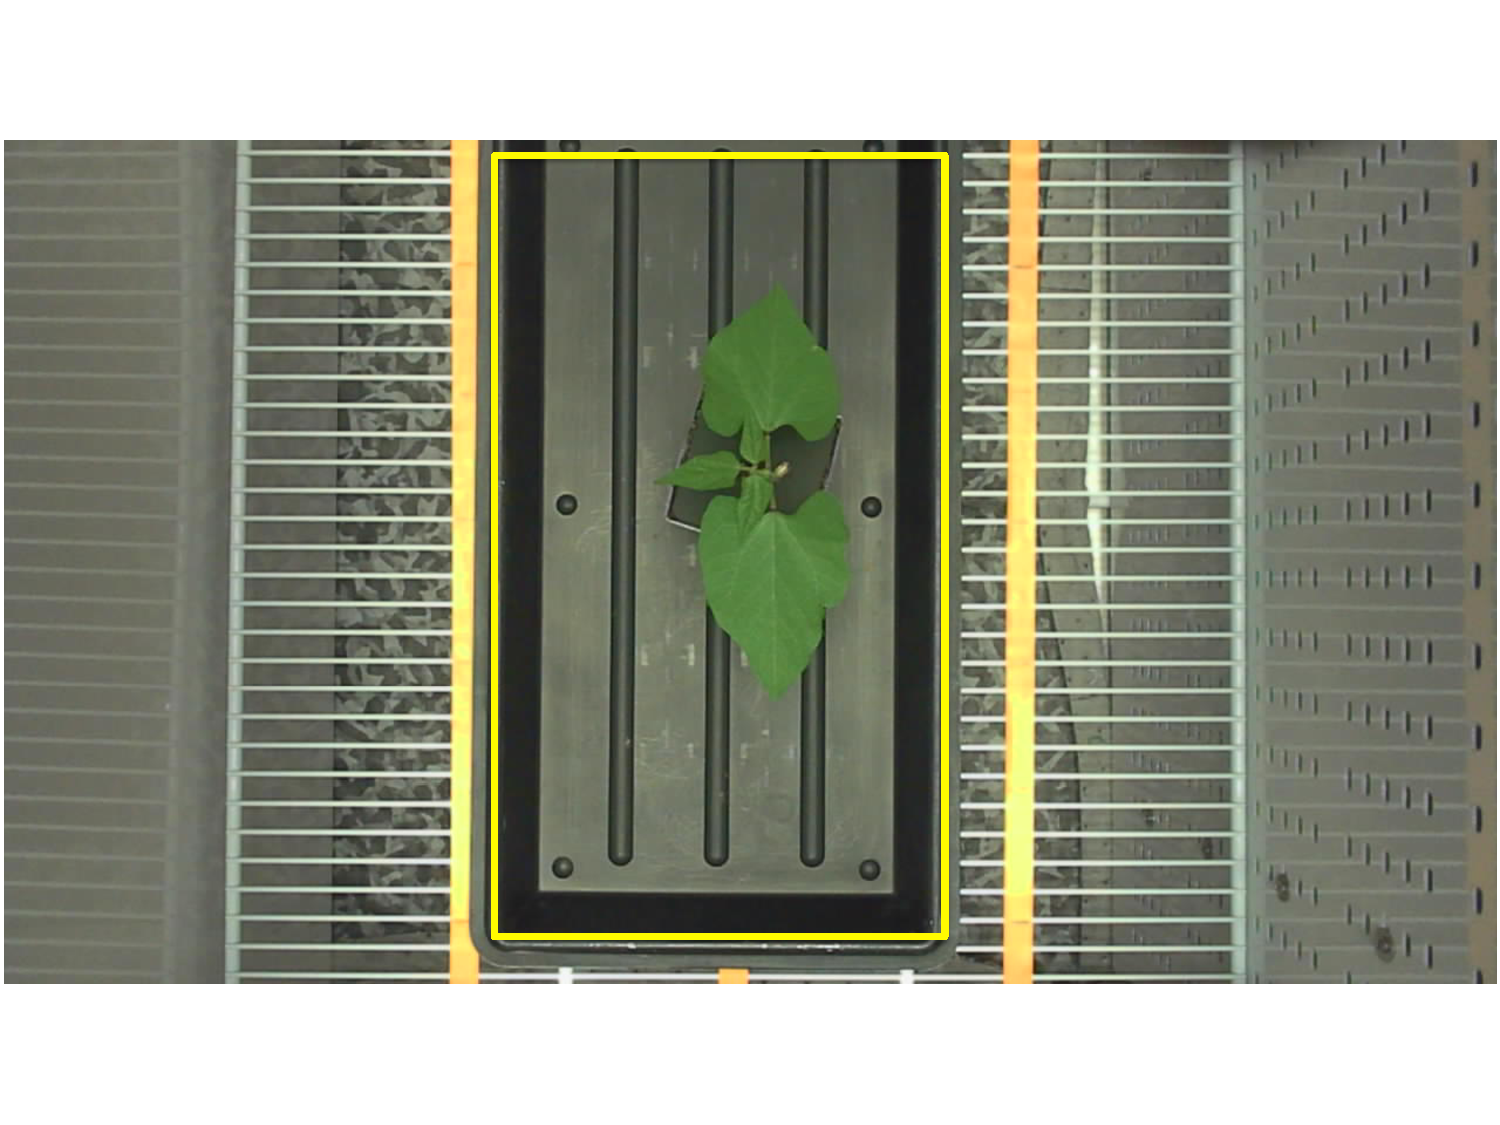
\includegraphics[width=.23\textwidth]{Figures/FourModalities/B_rgb}&
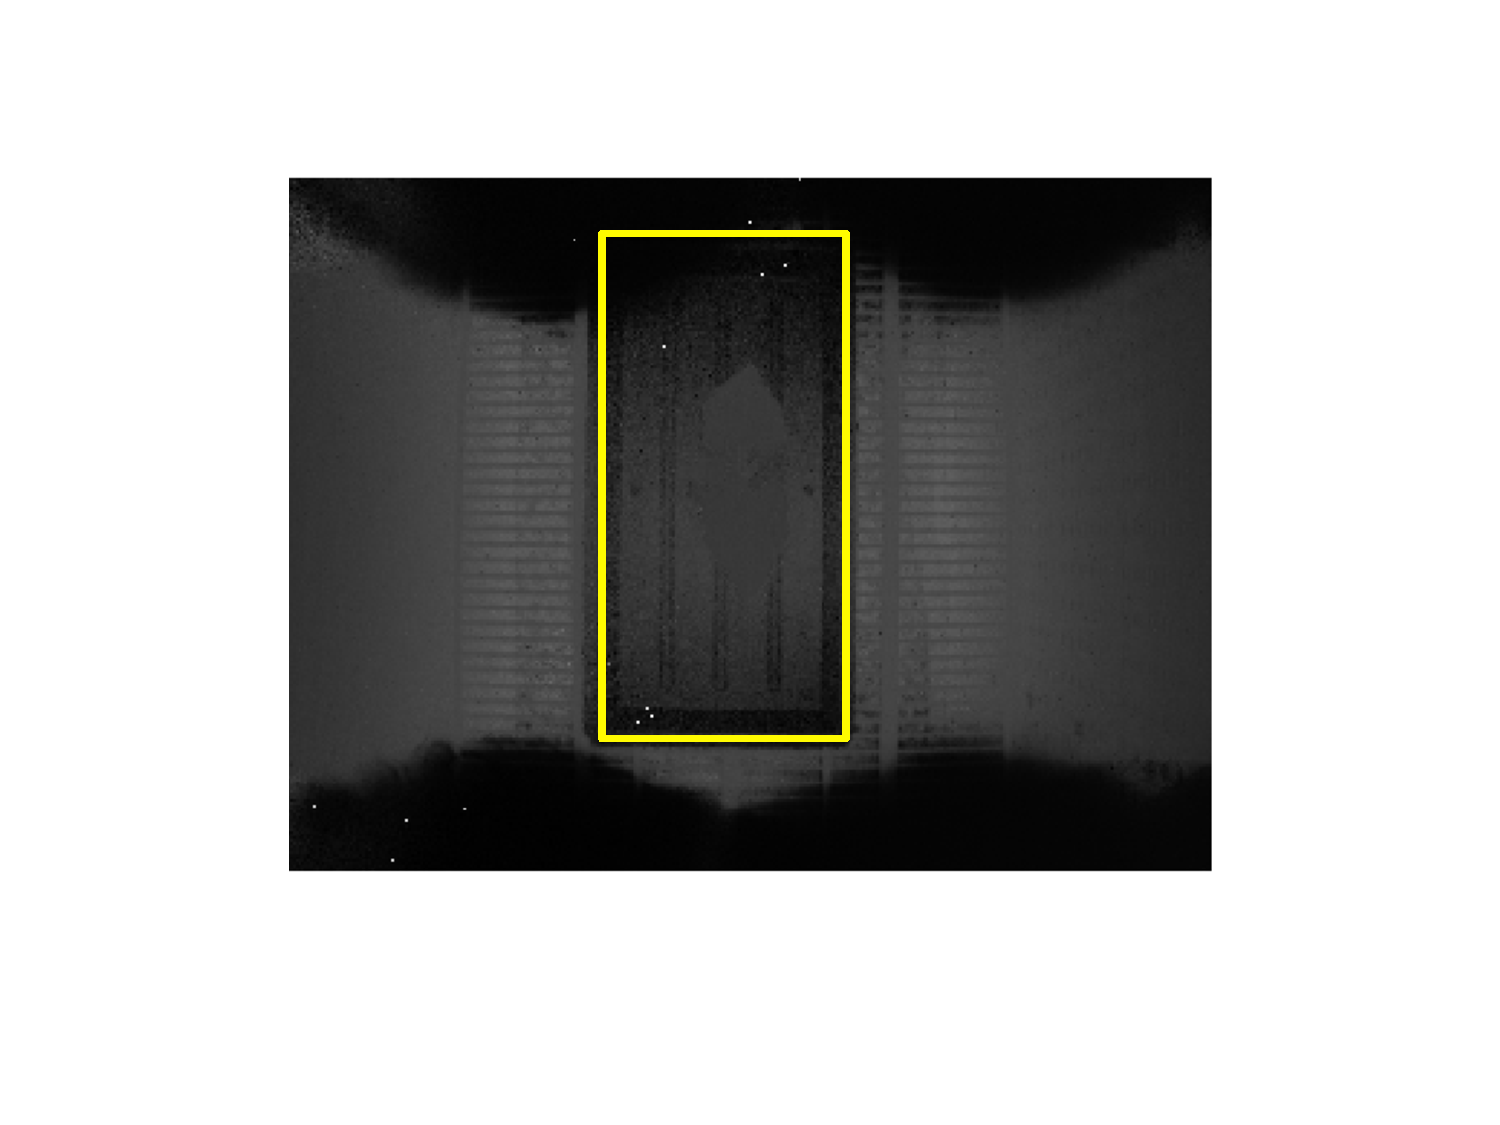
\includegraphics[width=.23\textwidth]{Figures/FourModalities/B_depth}&
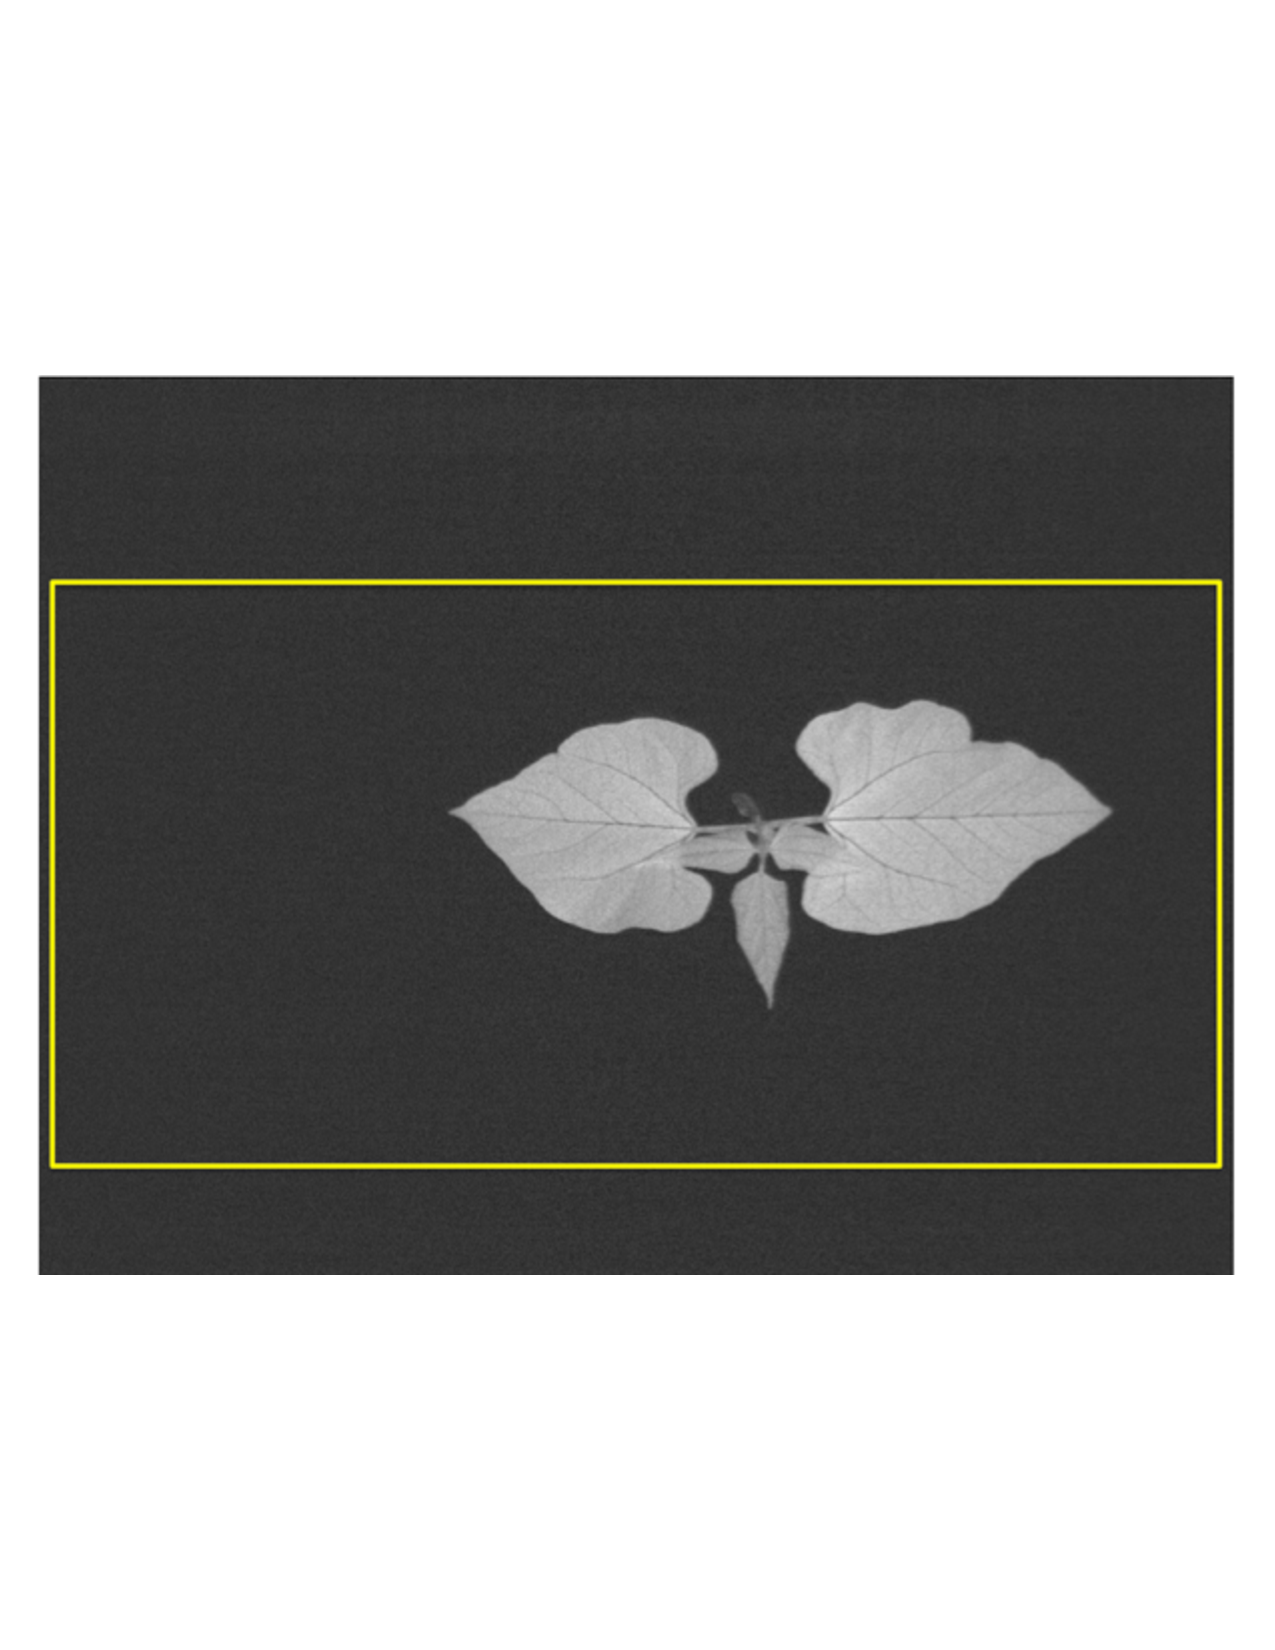
\includegraphics[width=.23\textwidth]{Figures/FourModalities/B_fmp}&
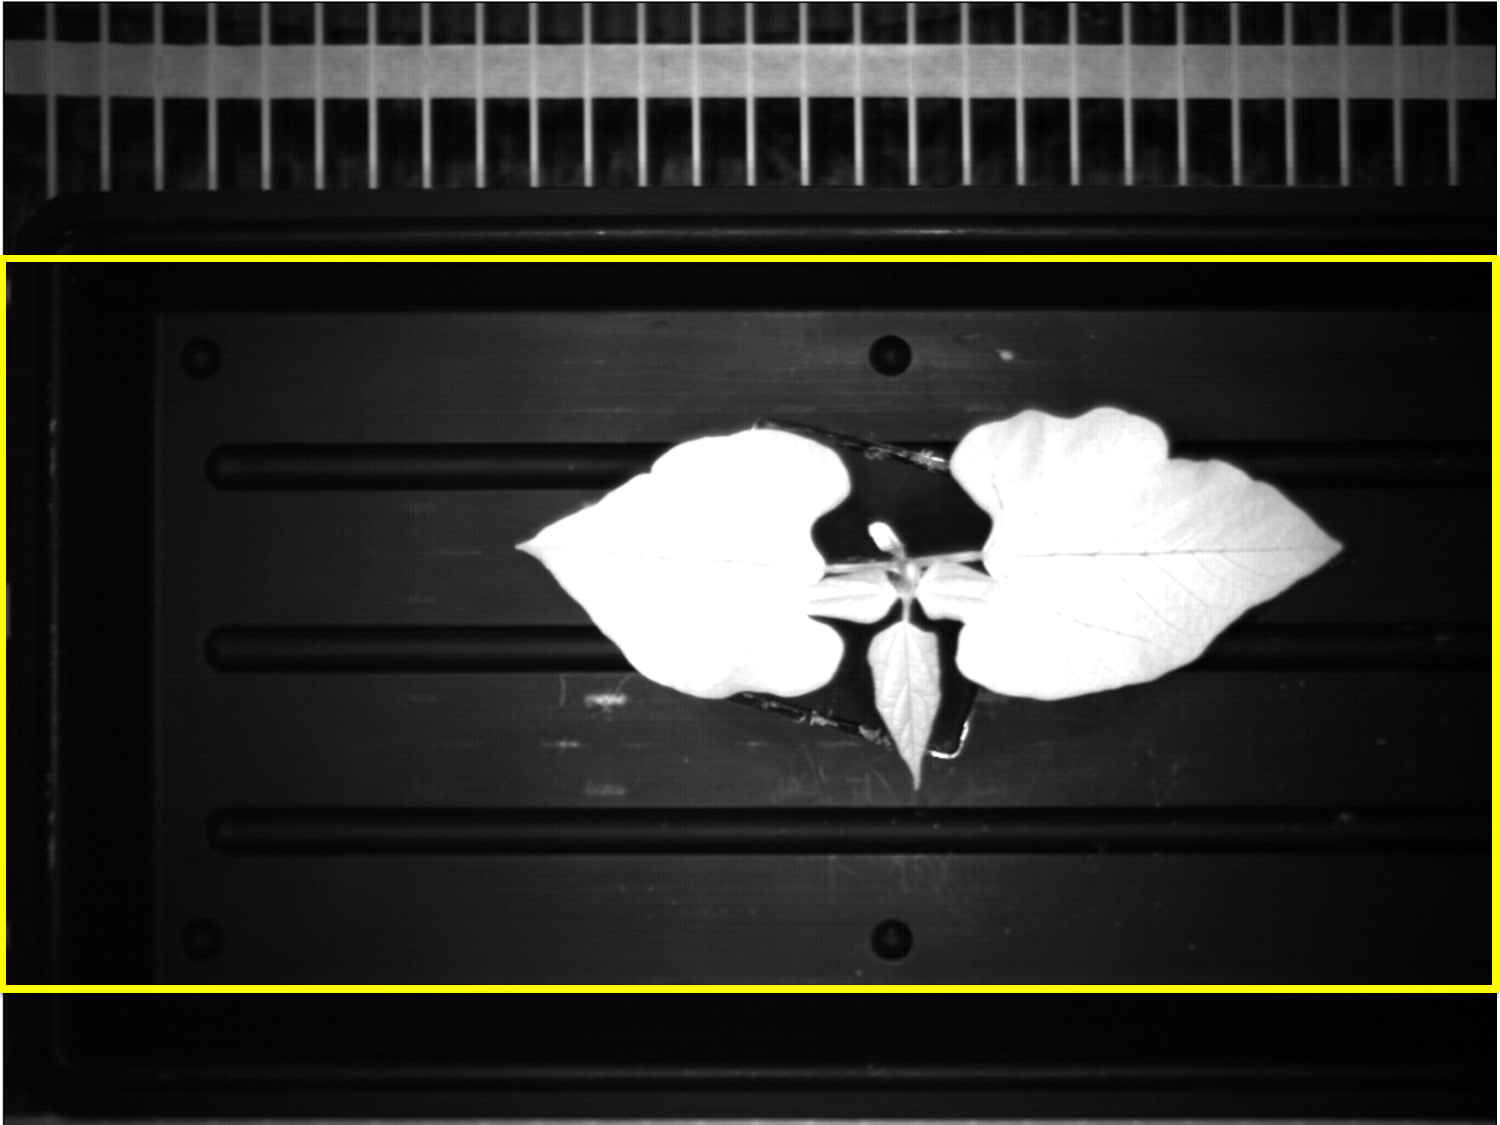
\includegraphics[width=.23\textwidth]{Figures/FourModalities/B_ir}\\
%(d) &
%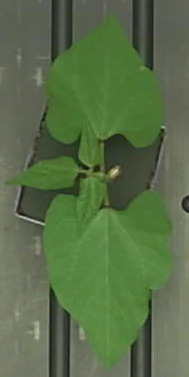
\includegraphics[width=.1\textwidth]{Figures/FourModalities/B1_rgb}&
%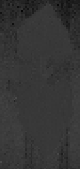
\includegraphics[width=.1\textwidth]{Figures/FourModalities/B1_depth}&
%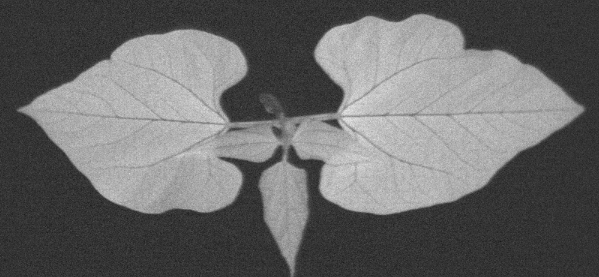
\includegraphics[width=.2\textwidth]{Figures/FourModalities/B1_fmp}&
%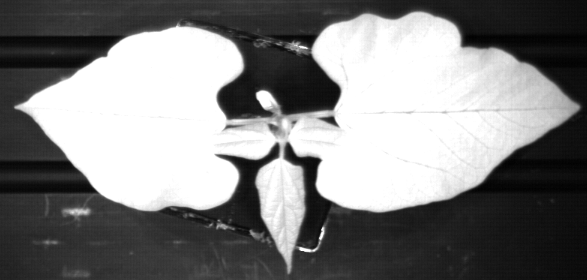
\includegraphics[width=.2\textwidth]{Figures/FourModalities/B1_ir}\\
%Bean: RGB & Bean: depth & Bean: fluorescence & Bean: IR \\
 & RGB & depth & fluorescence & IR\\
\end{tabular}
\caption{The multi-modality plant imagery database of MSU-PID. (a) four modalities of Arabidopsis; (b) zoom in view of Arabidopsis plant $1$; (c) four modalities of bean.}
\label{fig:fourmodality}
\end{centering}
\end{figure*}


Plants develop through a complex interaction between genotype and environment.
This determines their structure, functions, and thus performance such as yield or efficient usage of resources.
In order to understand the genetic basis of these economically important parameters, it is essential to quantitatively assess plant phenotypes and then identify the latent relationships to genotypes and environmental factors.
%
Plant visual phenotyping has been performed by farmers and breeders for more than $5,000$ years.
In the past, traditional phenotyping is based on experience and intuition, and is laborious~\cite{johannsenerblichkeit}.
Recent progresses in imaging sensor and computer vision technologies lead to the development of the ever-increasing new field of highly automated, non-destructive plant visual phenotyping~\cite{furbank2011phenomics,cruz2015depi}.
%Modern plant phenotyping is a comprehensive, large-scale assessment of plant traits such as growth, development, tolerance, resistance, architecture, physiology, ecology, yield, and metadata that form the basis for more complex parameters.
%
The objective of modern plant visual phenotyping is to analyze and categorize the morphological characteristics of plants, and thus accurately quantifying plant traits. %It advances crop yield improvement and enables the systematic study of the environmental plasticity of plants. %
In this interdisciplinary field, scientists employ various imaging sensors to capture plants and design advanced algorithms to automatically analyze the captured plant imagery, with the purpose of raising testable biological hypotheses to solve problems related to growth, development, stress tolerance, resistance, and so on.
%
%In old days, plant phenotyping was conducted through manual visual observation~\cite{Erblichkeit1903}. Today, motivated by the increasing lower cost and increasing diversity of imaging sensors technologies, image-based automatic plant visual phenotyping is quickly growing into a desirable and viable solution~\cite{furbank2011phenomics,cruz2015depi}.
%
A key advance in visual phenotyping is the capability to non-invasively capture plant traits, enabling continuous measurements that are necessary to monitor plants during growth and/or under stress conditions. 
It also increases the throughput of phenotyping experiments by eliminating destructive operations, which allows more genotypes or biological replicates to be examined under the same environmental conditions~\cite{fahlgren2015lights,walter2015plant}.

One goal of plant visual phenotyping is to accurately quantify plant traits, particularly those related to photosynthetic performance, growth, yield, and resilience to environmental stress.
For the approaches to be of practical, plants must be monitored continuously, over developmental time scales and under conditions that approximate the native environment (dynamic 'field' conditions)~\cite{fahlgren2015lights,walter2015plant}.
%
The capacity to identify and track individual leaves over time is important to clearly define phenotypic behaviors related to leaf-specific factors such as developmental age~\cite{schottler2015photosynthetic} and/or following the application of stress.
For example, decrease in the average photosynthetic efficiency ($\Phi_{II}$, quantum yield of photochemistry at photosystem II) of an Arabidopsis plant may reflect a heterogeneous distribution of $\Phi_{II}$ values across its entire photosynthetic surface area~\cite{oxborough2004imaging}.
In this case, mapping distributions to individual leaves can distinguish between a systemic (whole plant) effect and localization of the effect to subset leaves.
%
In addition, using more detailed information, such as leaf angles, height, and position as well as canopy density and size, it is possible to improve the estimation of total photosynthetic capacity over time (particularly for plants with more complex canopies, e.g., common bean or tobacco), since these factors influence absorption and availability of the light energy used to drive photosynthesis.

\begin{table*}[t!]
\centering
\begin{threeparttable}
\caption{Plant image databases.}
%\resizebox{12cm}{!} {
%\begin{tabular}{|l@{}|@{}c@{}|@{}c@{}|@{}c@{}|@{}c@{}|@{}c@{}|}
\begin{tabular}{l|c|c|c|c|c|c}
%\hline
%\multirow{2}{*}{Database}& \multirow{2}{*}{Modality} & \multirow{2}{*}{Applications}\tnote{a} & \multirow{2}{*}{Plant Type} & Subject/ &Total & Labeled \\
%& & & & Classe \# & Image \# & Image \# \\ \hline
%Swedish leaf~\cite{soderkvist2001computer} & Scaned leaf & LC& Swedish trees & $15$ & $1,125$ & $1,125$ \\ \hline
%Flavia~\cite{wu2007leaf} & RGB & LC& Leaves & $32$ & $2,120$ & $2,120$ \\ \hline
%Leafsnap~\cite{kumar2012leafsnap} & RGB & LC& USA trees & $184$ & $29,107$ & $29,107$ \\ \hline
%Crop/weed~\cite{haug2014crop} & RGB &Weed detection & Crop/weed & $2$ & $60$ & $60$ \\ \hline
%\multirow{2}{*}{LSC~\cite{haug2014crop}} & \multirow{2}{*}{RGB} & \multirow{2}{*}{LS, LO} & Arabidopsis & $43$ & $6287$ & $201$ \\ \cline{4-7}
%& & & Tobacco & $80$ & $165,120$ & $83$ \\ \hline
%\multirow{2}{*}{MSU-PID} & fluorescence, & LS, LO, & Arabidopsis & $16$ & $2304\times 4$ & $576\times 4$ \\ \cline{4-7}
%& IR, RGB, depth & LA, LT & Bean & $5$ & $350\times 4$ & $175\times 4$ \\ \hline
%\hline
\hline
\multirow{2}{*}{Database}& \multirow{2}{*}{Modality} & \multirow{2}{*}{Applications}\tnote{a} & \multirow{2}{*}{Plant Type} & Subject/ &Total & Labeled \\
& & & & Classe \# & Image \# & Image \# \\ \hline
Swedish leaf & \multirow{2}{*}{Scaned leaf} & \multirow{2}{*}{LC} & \multirow{2}{*}{Swedish trees} & \multirow{2}{*}{$15$} & \multirow{2}{*}{$1,125$} & \multirow{2}{*}{$1,125$} \\
~\cite{soderkvist2001computer} & & & & & & \\ \hline
Flavia & \multirow{2}{*}{RGB} & \multirow{2}{*}{LC} & \multirow{2}{*}{Leaves} & \multirow{2}{*}{$32$} & \multirow{2}{*}{$2,120$} & \multirow{2}{*}{$2,120$} \\
~\cite{wu2007leaf} & & & & & & \\ \hline
Leafsnap & \multirow{2}{*}{RGB} & \multirow{2}{*}{LC} & \multirow{2}{*}{USA trees} & \multirow{2}{*}{$184$} & \multirow{2}{*}{$29,107$} & \multirow{2}{*}{$29,107$} \\
~\cite{kumar2012leafsnap} & & & & & & \\ \hline
Crop/weed & \multirow{2}{*}{RGB} & \multirow{2}{*}{Weed detection} & \multirow{2}{*}{Crop/weed} & \multirow{2}{*}{$2$} & \multirow{2}{*}{$60$} & \multirow{2}{*}{$60$} \\
~\cite{haug2014crop} & & & & & & \\ \hline
LSC & \multirow{2}{*}{RGB} & \multirow{2}{*}{LS, LO} & Arabidopsis & $43$ & $6,287$ & $201$ \\ \cline{4-7}
~\cite{haug2014crop} & & & Tobacco & $80$ & $165,120$ & $83$ \\ \hline
\multirow{2}{*}{MSU-PID} & fluorescence, & LS, LO, & Arabidopsis & $16$ & $2,160\times 4$ & $576\times 4$ \\ \cline{4-7}
& IR, RGB, depth & LA, LT & Bean & $5$ & $325\times 4$ & $175\times 2$ \\ \hline
\hline
\end{tabular}
%}
\begin{tablenotes}
\footnotesize
\item[a] The abbreviation in ``Applications'' column is defined as Leaf Classification (LC), Leaf Segmentation (LS), Leaf Counting (LO), Leaf Alignment (LA), and Leaf Tracking (LT).
\end{tablenotes}
\end{threeparttable}
\label{tab:database}
\end{table*}

Due to diverse variations of leaf shape, appearance, layout, growth and movement, plant image analysis is a non-trivial computer vision task~\cite{Minervini2015}.
In order to develop advanced computer vision algorithms, image databases that are well representative of this application domain is highly important.
In fact, computer vision research lives on and advances with databases, as evidenced by the successful databases in the field (e.g., FERET~\cite{Phillips2000} and LFW~\cite{LFW}).
However, the publicly available databases for plant phenotyping are still very limited, with the only exception of LSC database~\cite{scharr2014annotated}, which, nevertheless, has its own limitations on the type of images (RGB only) and is only suitable for a small set of plant image analysis applications.


To facilitate future research on plant image analysis, as well as remedy the limitation of existing databases in the field, this paper presents a newly collected multi-modality Plant Imagery Database through an interdisciplinary effort at Michigan State University (MSU), which is termed ``MSU-PID''.
As illustrated in Figure~\ref{fig:fourmodality}, the MSU-PID database includes the imagery of two types of plants (Arabidopsis and bean, both are widely used in plant research) captured by four types of imaging sensors, i.e., fluorescence, infrared (IR), RGB color, and depth.
All four sensors are synchronized and are programmed to periodically capture imagery data for multiple consecutive days.
Checkerboard-based camera calibration is performed on each modality providing intrinsic camera parameters and poses.  In addition explicit correspondence between the pixels of {\it any} two modalities is obtained using an homographic warping of a plane through the Arabidopsis plants.


The type and amount of manual labels on a database is a critical enabler to the potential applications of the database.
For a subset of the MSU-PID database, we manually label the groundtruth regarding the leaf identification number, locations of leaf tips, and leaf segments.
As a result, MSU-PID is suitable for a number of applications, including $1)$ {\it leaf segmentation} that aims at estimating the correct segmentation mask of each leaf in an image, $2)$ {\it leaf counting} that estimates the correct number of leaves within a plant, $3)$ {\it leaf alignment} that aligns the two tips of each leaf -- the cornerstone of the leaf structure, and $4)$ {\it leaf tracking} that is designed to track each leaf over time.
Finally, to provide a performance baseline for future research and comparison, we apply our automatic leaf segmentation framework~\cite{yin2014a,yin2014b} to the Arabidopsis imagery and demonstrate the unique challenge of image analysis on this database.

In summary, this paper and our database have made the following main contributions.
\begin{itemize}
\item MSU-PID is the first {\it multi-modality} plant image database. This allows researchers to study the strength and weakness of individual modality, as well as their various combinations in plant image analysis.
\item Our unique imaging setup and the variety of manual labels make MSU-PID an ideal candidate for evaluating a diverse set of plant image analysis applications including leaf segmentation, leaf counting, leaf alignment, leaf tracking, and potentially leaf growth prediction and $3$D leaf reconstruction.
\end{itemize}




\section{Prior Work}
\label{sec:prior}

Databases drive computer vision research.
Hence, it is always important to develop and promote properly captured databases in the vision community.
While there is a clear desire to apply computer vision to plant image analysis, the lack of publicly available plant image databases has been an obstacle for further study and development.

We summarize existing publicly available databases that are most related to our work in Table~\ref{tab:database}.
In terms of potential applications of these databases, they can be categorized into two types.
The first type is for the general purpose of recognizing a particular species of tree or plant.
The Swedish leaf database~\cite{soderkvist2001computer} is probably the first leaf database even though the images are captured by scanners.
The Flavia database~\cite{wu2007leaf} is considerably larger and a neural network is utilized to train a leaf classifier.
The most recent Leafsnap project~\cite{kumar2012leafsnap} is an impressive effort that includes a very large dataset of leaves for $184$ tree types.
A mobile phone application is also developed to make the leaf classification system portable.
Finally, the crop/weed image database~\cite{haug2014crop} is captured by a robot in the real field, and used for the classification of crop vs. weed.
Note that except for~\cite{haug2014crop} where images are captured in the wild for a large area of plant, other databases in this type normally capture only a {\it single} leaf in a relatively constrained imaging environment.
Therefore, the challenging problem of leaf segmentation has been bypassed.
% Note that in this type of databases, normally only a {\it single} leaf is imaged in a relatively constrained imaging environment and as a result, the challenging problem of leaf segmentation has been bypassed.

The second type of databases is for plant phenotyping, where it is important to capture plant images without interfering the growth of plants.
Thus, non-destructive imaging approaches are taken and the entire plant is imaged. 
The LSC database~\cite{scharr2014annotated} is the most relevant one to our database.
It captures a large set of RGB images for Arabidopsis and tobacco plants.
The provided manual labels allow the evaluation of leaf segmentation and leaf counting.
In comparison, our MSU-PID database utilizes four sensing modalities in the data capturing, each providing different aspects of plant visual appearance.
Our diverse manual labels also enable us to develop algorithms for additional applications such as leaf tracking and leaf alignment.

%One of our data modalities is dense depth measurement. This has been a component of a number of recent non-plant RGB-D databases designed for object recognition~\cite{Lai2011}, scene segmentation~\cite{Silberman2011}, human analysis~\cite{Sung2011,Barbosa:reid12}, and mapping~\cite{sturm12iros}. By including dense depth for a plant database we anticipate enabling development of new 3D plant shape analysis algorithms.

The four sensing modalities in MSU-PID provide unique opportunities to comprehensively characterize plant morphological and physiological phenotypes. 
The use of chlorophyll fluorescence at $730nm$ to $750nm$ as a tool for evaluating photosynthetic performance is well established~\cite{baker2008chlorophyll}, and against non-(chlorophyll)fluorescent background clearly defines photosynthetically active leaf area.
The depth measurement has been a component of a number of recent non-plant RGB-D databases designed for object recognition~\cite{Lai2011}, scene segmentation~\cite{Silberman2011}, human analysis~\cite{Sung2011,Barbosa:reid12}, and mapping~\cite{sturm12iros}. 
By including depth map for a plant database, we anticipate enabling development of new $3$D plant canopy analysis algorithms and thus probing the total energy intake and storage.
Near infrared (IR) reflectance has been used by others to detect water content in leaves~\cite{chen2014dissecting}.  
However, it may also be useful in determining leaf angle and curvature.  
Furthermore, since imaging occurs at a wavelength that is effectively non-absorbing for photosynthesis or known light receptors~\cite{butler1964actton,eskins1992light} in plants, it can be used for imaging during the night cycle to observe night time leaf expansion or in some cases circadian movements~\cite{mcclung2006plant}.








\section{Data Collection}\label{sec:2}

\subsection{Plants}

\section{Data Collection}
\label{sec:2}

\subsection{Plants and Growth Conditions}

{\it Arabidopsis thaliana} (ecotype Col-$0$) plants were grown at $20^{\circ}C$, under a $16~hr$ : $8~hr$ day-night cycle with a daylight intensity set at $100~\mu mol~photons~m^{-2} s^{-1}$.
%
Black bean plants ({\it Phaseolus vulgaris L.}) of the cultivar Jaguar, were grown under a $14~hr$ : $10~hr$ day-night cycle with day and night temperatures of $24^{\circ}C$ and $18^{\circ}C$ respectively, and a daylight intensity set at $200~\mu mol~photons~m^{-2} s^{-1}$.
%
Note that the bean plants were watered with half-strength Hoaglands solution three times per week.

In all cases, seeds were planted in soil covered with a black foam mask in order to minimize the fluorescence background from algal growth.
%
Two-week-old plants ({\it Arabidopsis} and bean) were transferred to imaging chambers and allowed to acclimate (\todo{Jeff: Please define ``acclimate" as in Comment $37$}) for $24$ hours to the LED lighting before the start of the data collection.
Growth conditions as described above were maintained for each set of plants for the duration of image collection.


\subsection{Hardware Setup}

\begin{figure}
  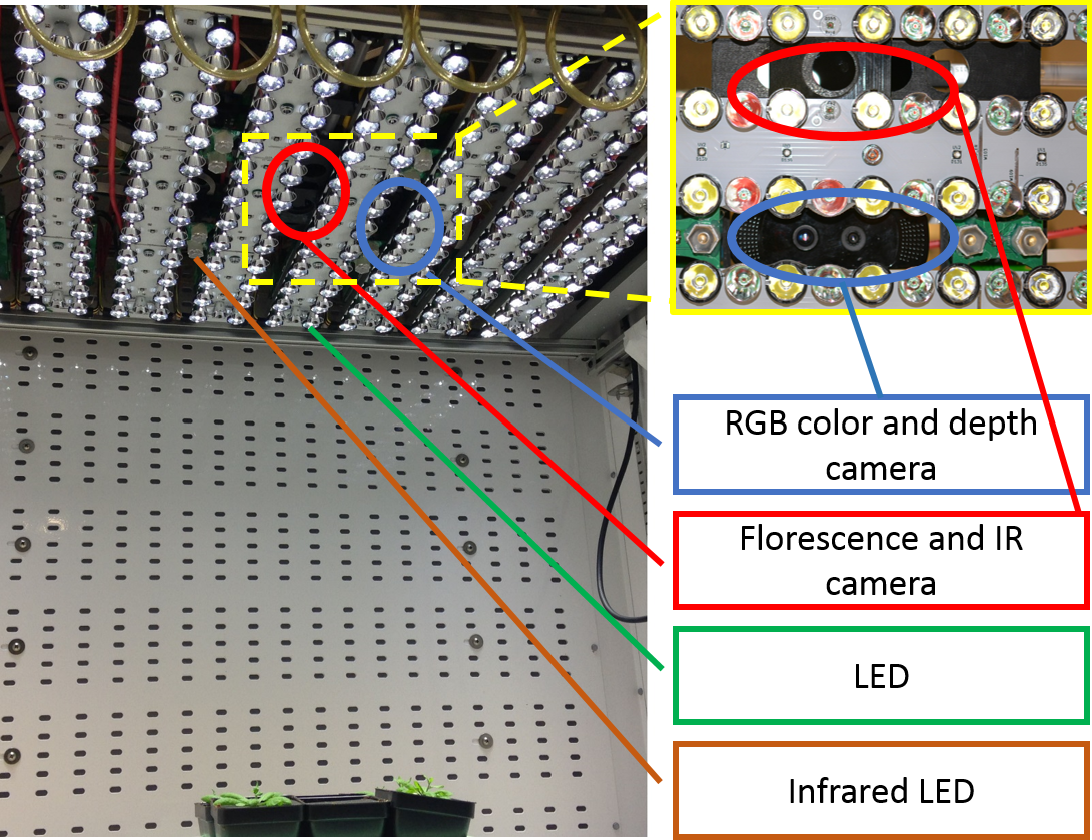
\includegraphics[width=\linewidth,trim=55 100 200 70,clip]{Figures/hardware}
\caption{The hardware setup for our data collection.}
\label{fig:hardware}
\end{figure}

\subsection{Hardware Setup}

In this section, we introduce the hardware used for capturing fluorescence, IR, RGB color, and depth imagery data for both plants.
Figure~\ref{fig:hardware} illustrates the hardware and imaging setup used in our data collection.

\subsubsection{Fluorescence and IR Images}
Chlorophyll a fluorescence images were captured once every hour during the daylight period in a growth chamber~\cite{cruz2015depi}.
A set of $5$ images were captured using a Hitachi KP-F145GV CCD camera (Hitachi Kokusai Electric America Inc., Woodbury, NY) outfitted with an infrared long pass filter (Schott Glass RG-9, Thorlabs, Newton, NJ), during a short period ($<400~ms$) of intense light saturating to photosynthesis ($>10,000~\mu mol~photons~m^{-2} s^{-1}$) provided by an array of white Cree LEDs (XMLAWT, 5700K color temperature, Digi-Key, Thief River Falls, MN) collimated using a $20~mm$ Carclo Lens (10003, LED Supply, Lakewood, CO).
%
Chlorophyll a fluorescence was excited using monochromatic red LEDs (Everlight $625~nm$, ELSH-F51R1-0LPNM-AR5R6, Digi-Key), collimated using a Ledil reflector optic ($C11347\_REGINA$, Mouser Electronics, Mansfield, TX) and pulsed for $50~\mu s$ during a brief window when the white LEDs were electronically shuttered.
In addition, a series of $5$ images were also collected in the absence of the excitation light for artifact subtraction.

Infrared images were collected once every hour with the same camera and filter used for chlorophyll a fluorescence.
Pulses of $940~nm$ light were provided by an array of OSRAM LEDs (SFH 4239, Digi-Key), collimated using a Polymer Optics lens (Part no. 170, Polymer Optics Ltd., Berkshire, England).
Since $940~nm$ light does not influence plant development or drive photosynthesis, images were also collected during the night period.
Sets of $15$ images were collected for averaging, in the absence of saturating illumination.
As with chlorophyll a fluorescence, images were captured in the absence of $940~nm$ light for artifact subtraction.



\subsubsection{RGB Color and Depth Images} %This section describes characterizes the data from this sensor, particularly the depth data.

The RGB color and depth images were collected using a Creative Senz3D sensor~\cite{nguyen2015vietnamese}. The sensor contains both a $1280 \times 720$ color camera directed parallel to, and separated by roughly $25~mm$ from, a depth camera which has a resolution of $320\times240$ pixels.
The depth sensor uses a flash near IR illuminator and measures the time-of-flight of the beam at each pixel to obtain dense depth estimates along with an IR reflectance at each pixel.

There are a number of limitations to the depth sensor that become the sources of depth errors.
The primary measurement limitation on the range-to-target is the strength of the reflected beam.
As a result, dark, matt surfaces are measured reliably only at a close range on the order of $20$ or $30~cm$.
Highly reflective surfaces also pose problems with direct reflections leading to saturation and highly unreliable depths.
In addition reflective surfaces at grazing angles are less reliably measured since little signal is reflected.
Fortunately the primary goal of the depth measurements are to obtain leaf depths, and plants provide good, roughly Lambertian, reflections of IR~\cite{Chelle2006219}.  Thus the depth pixels that are most reliable and are of most use are those that fall on plant foliage.

% For one-column wide figures use
\begin{figure}
\begin{tabular}{c}
  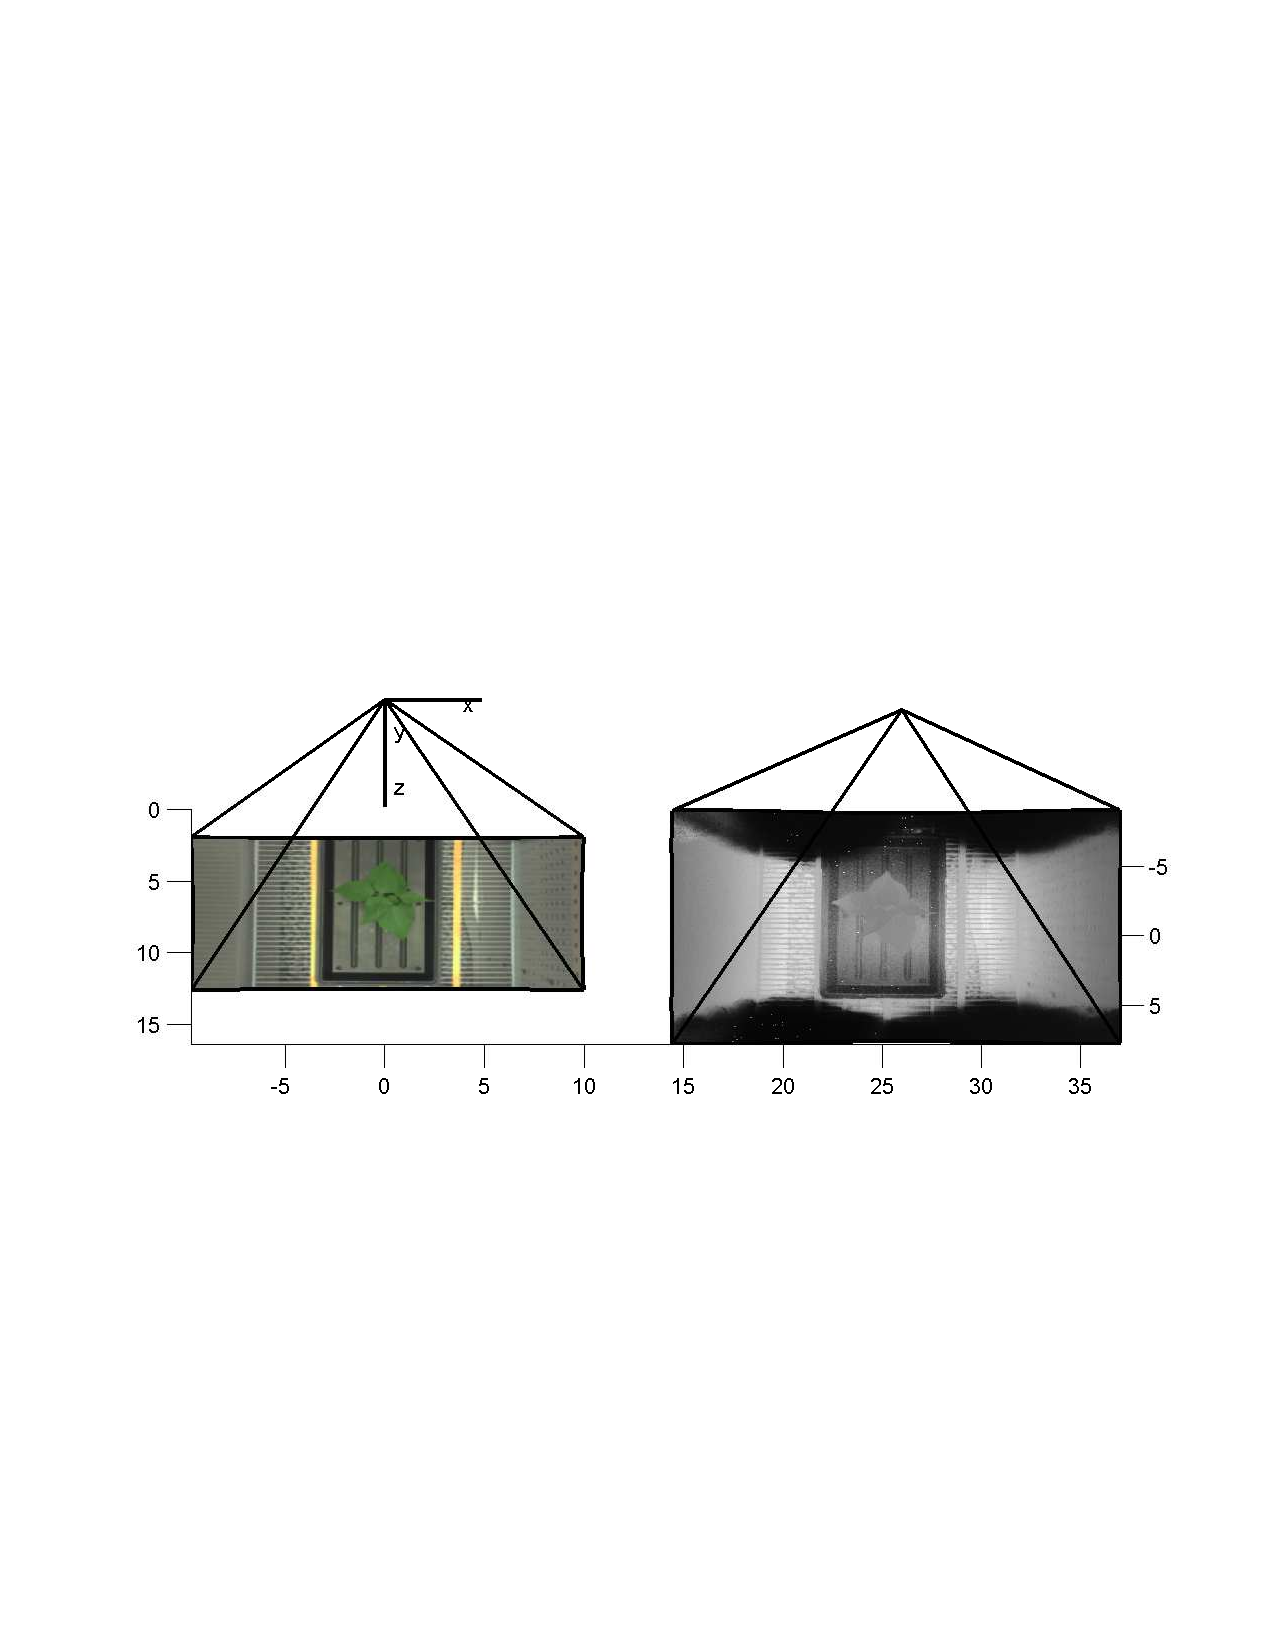
\includegraphics[width=\linewidth,trim=120 240 80 300,clip]{Figures/CameraConfiguration} \\
  ($a$)\\
  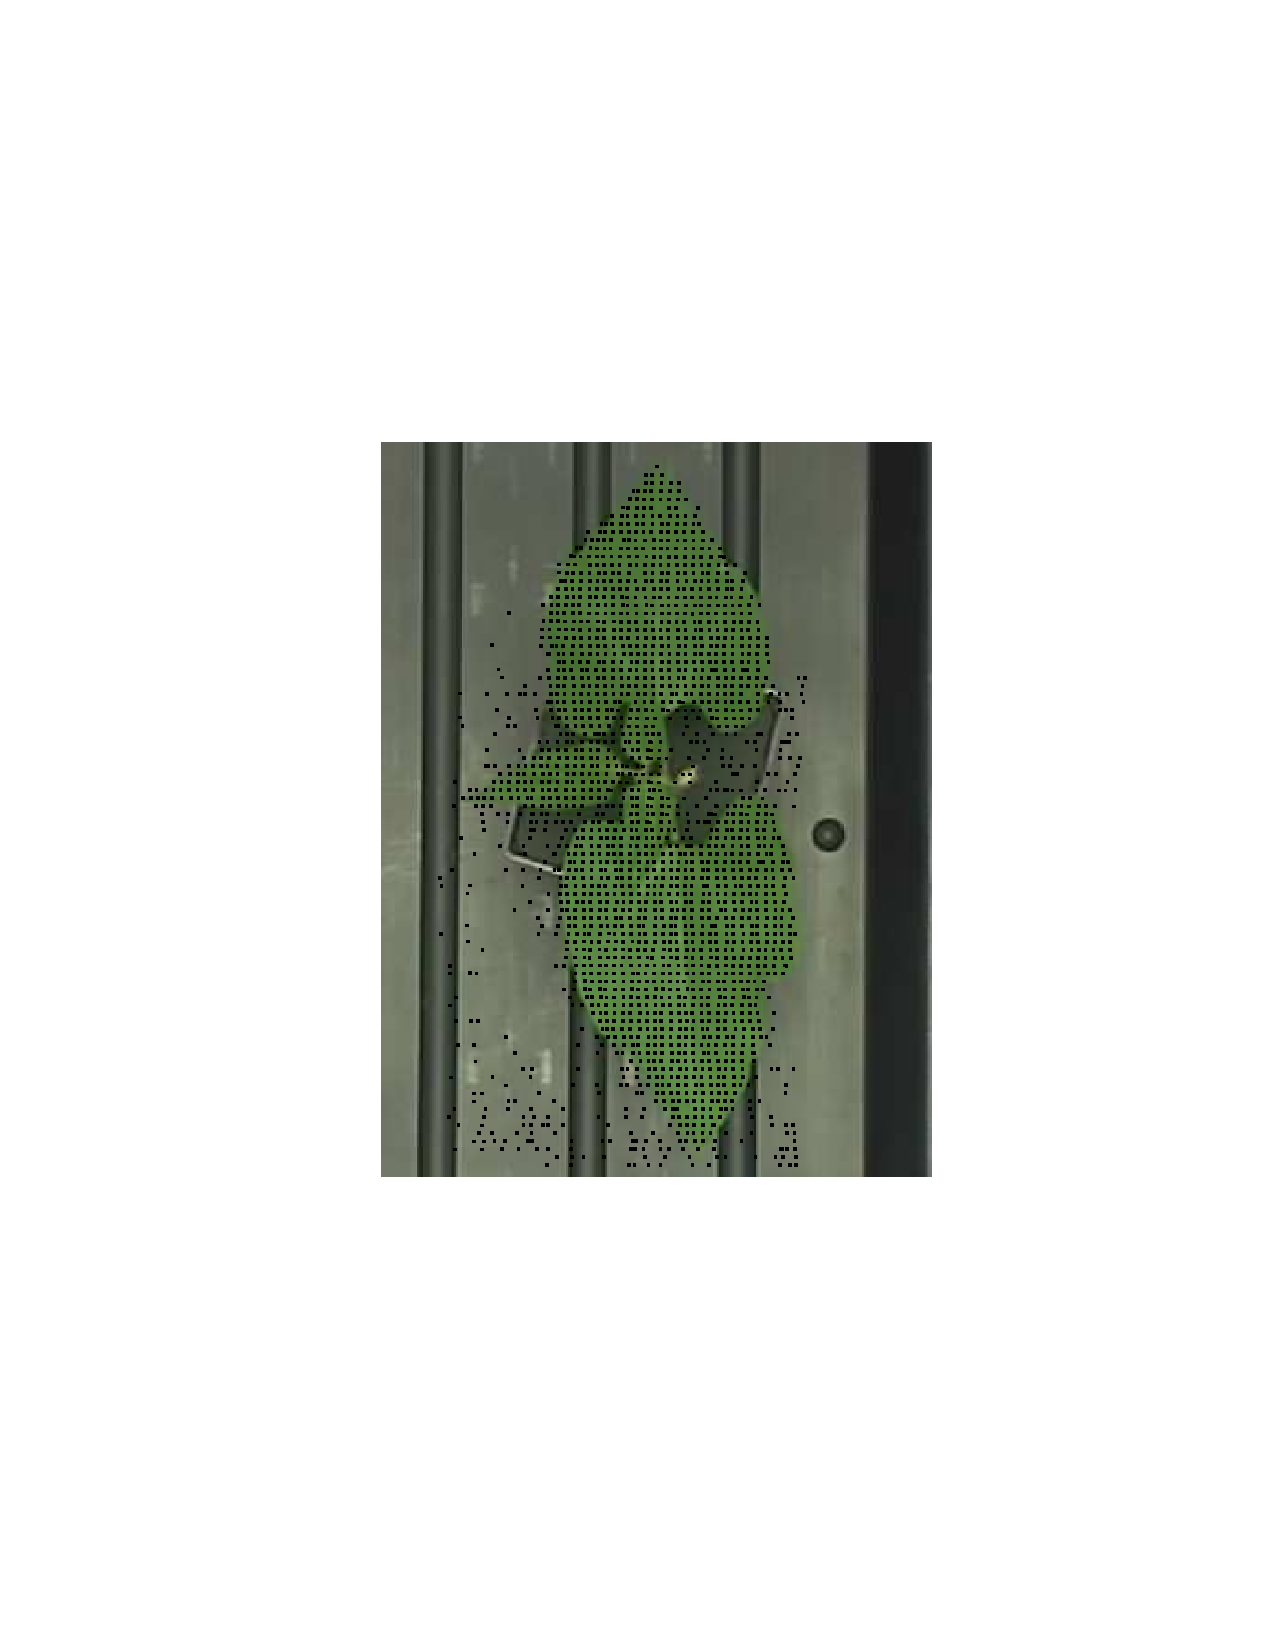
\includegraphics[width=0.65\linewidth,trim=175 220 162 180, clip,angle=-90,origin=c]{Figures/DepthOnBeanRGB} \vspace{-10mm} \\
  ($b$)\\
\end{tabular}
\caption{($a$)A plot of the three cameras showing their relative configuration and fields of view as obtained through calibration.  Units are in $mm$, apart from the size of the images which are scaled and plotted at equal resolution.  The optical center of the color camera (left-most) defines the world coordinate system.  Close to it is the depth camera having much lower resolution.  The right-most camera is the combined fluorescent and IR camera. ($b$) $3$D points from the depth camera are projected along their rays into the world coordinates and then projected into the color and fluorescent camera images.  This shows the projection into the color image (with $90^{\circ}$ rotation for economical use of space).  Only points in a rectangular region around the plant in the depth image are selected, and these are further filtered by eliminating points with high standard deviation.  An algorithm requiring only $3$D points on the plant could select only those that fall on the leaf pixels.}
\label{fig:CameraConfiguration}
\end{figure}

The imagery data were collected once every hour.
These include the fluorescent image, the IR reflectance image with the same camera, the color image, the $3$D depth and a confidence image.
The $3$D depth image is built from the depth sensor by transforming the points into the world coordinates and is expressed in the unit of $mm$.
The confidence image is the standard deviation of the depth pixels.
This is useful for identifying pixels at depth discontinuities that are unreliably detected and result in large standard deviations.


\begin{figure}
\centering
  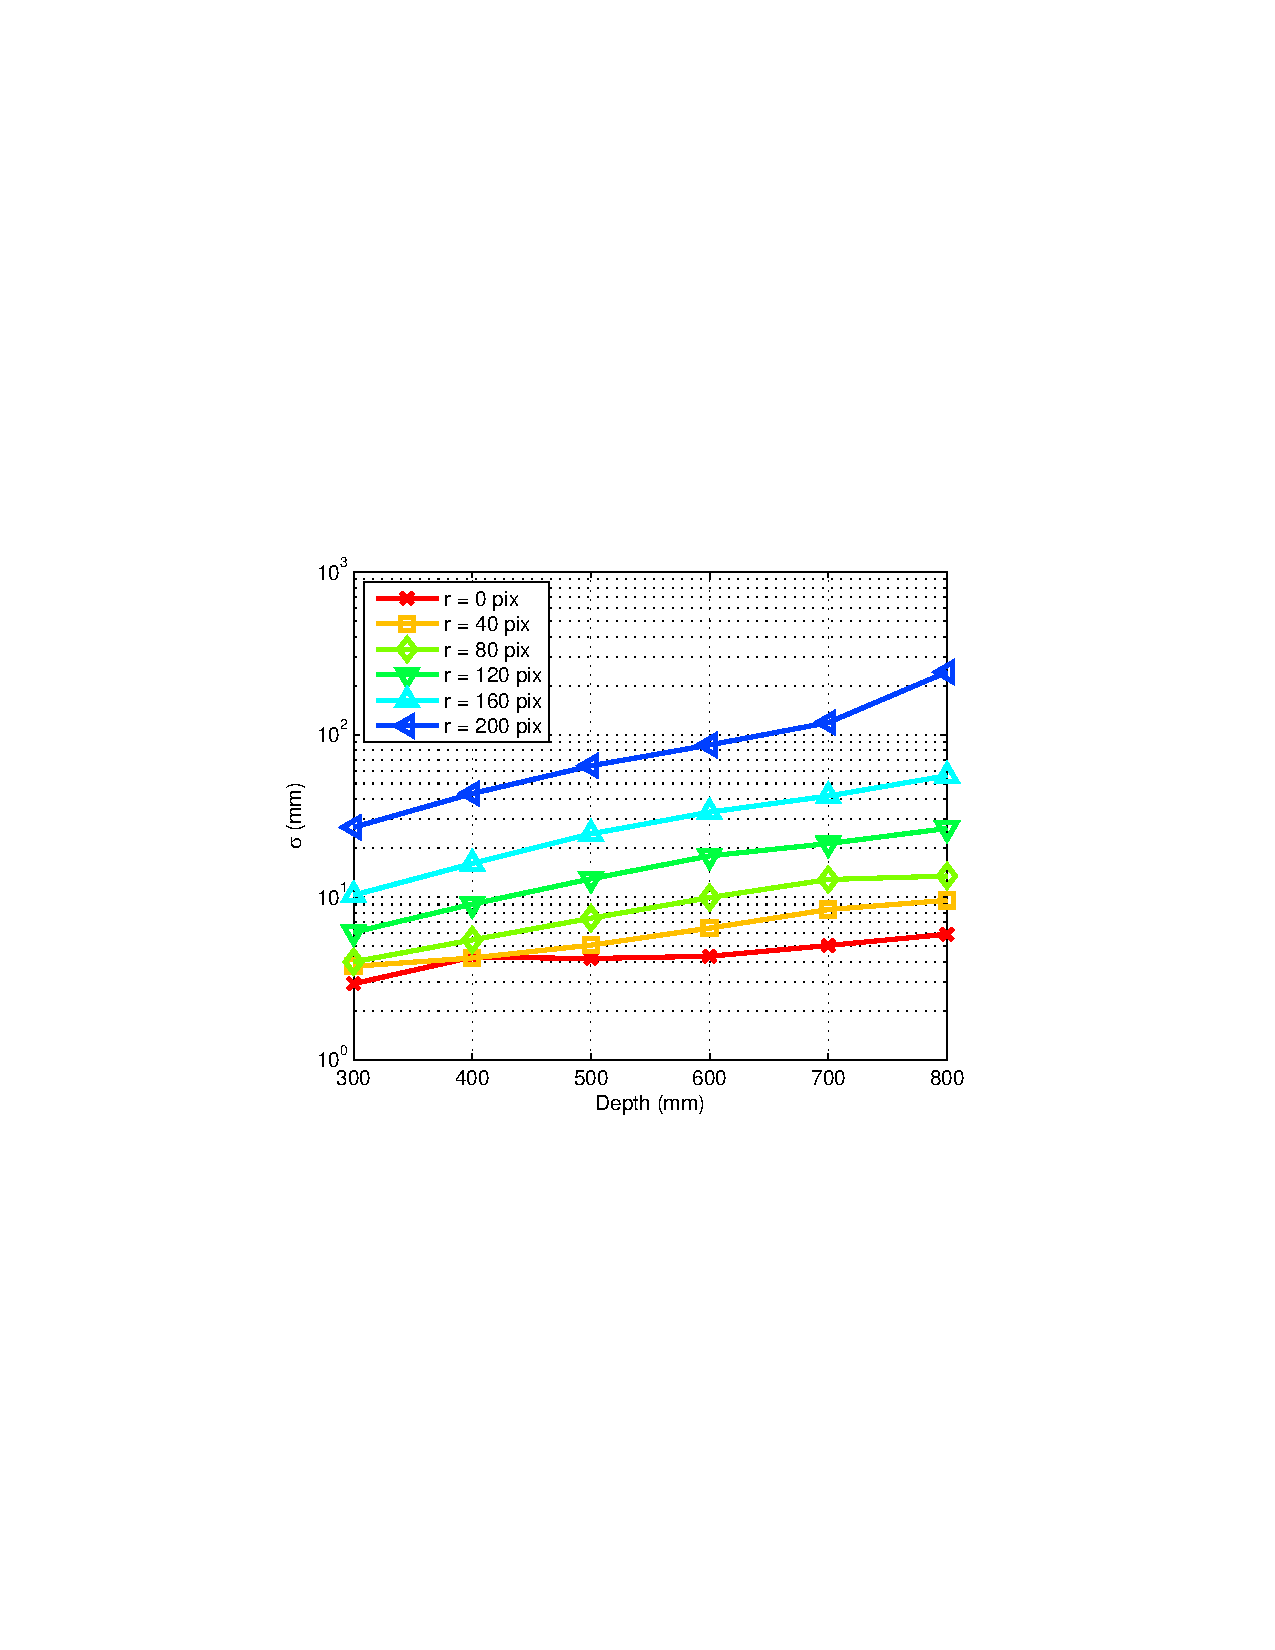
\includegraphics[height=5.9cm,trim=110 250 60 260,clip]{Figures/SigmaRadius} \\
\caption{Noise analysis for a depth camera obtained by imaging a flat surface at various depths.  We found that the standard deviation, $\sigma_I(d,r)$ from Eq. (\ref{eq:sigma}) of the pixel depth measurements had a large dependency on both the target depth, $d$, and the pixel radius, $r$, from the image center, and these are plotted.  A radius of $0$ pixels is the image center, and of $200$ pixels corresponds to the corners of the depth camera, which can be seen to have far larger standard deviation than at the image center for the same depth. }
\label{fig:Noise}
\end{figure}



% For one-column wide figures use
\begin{figure}
  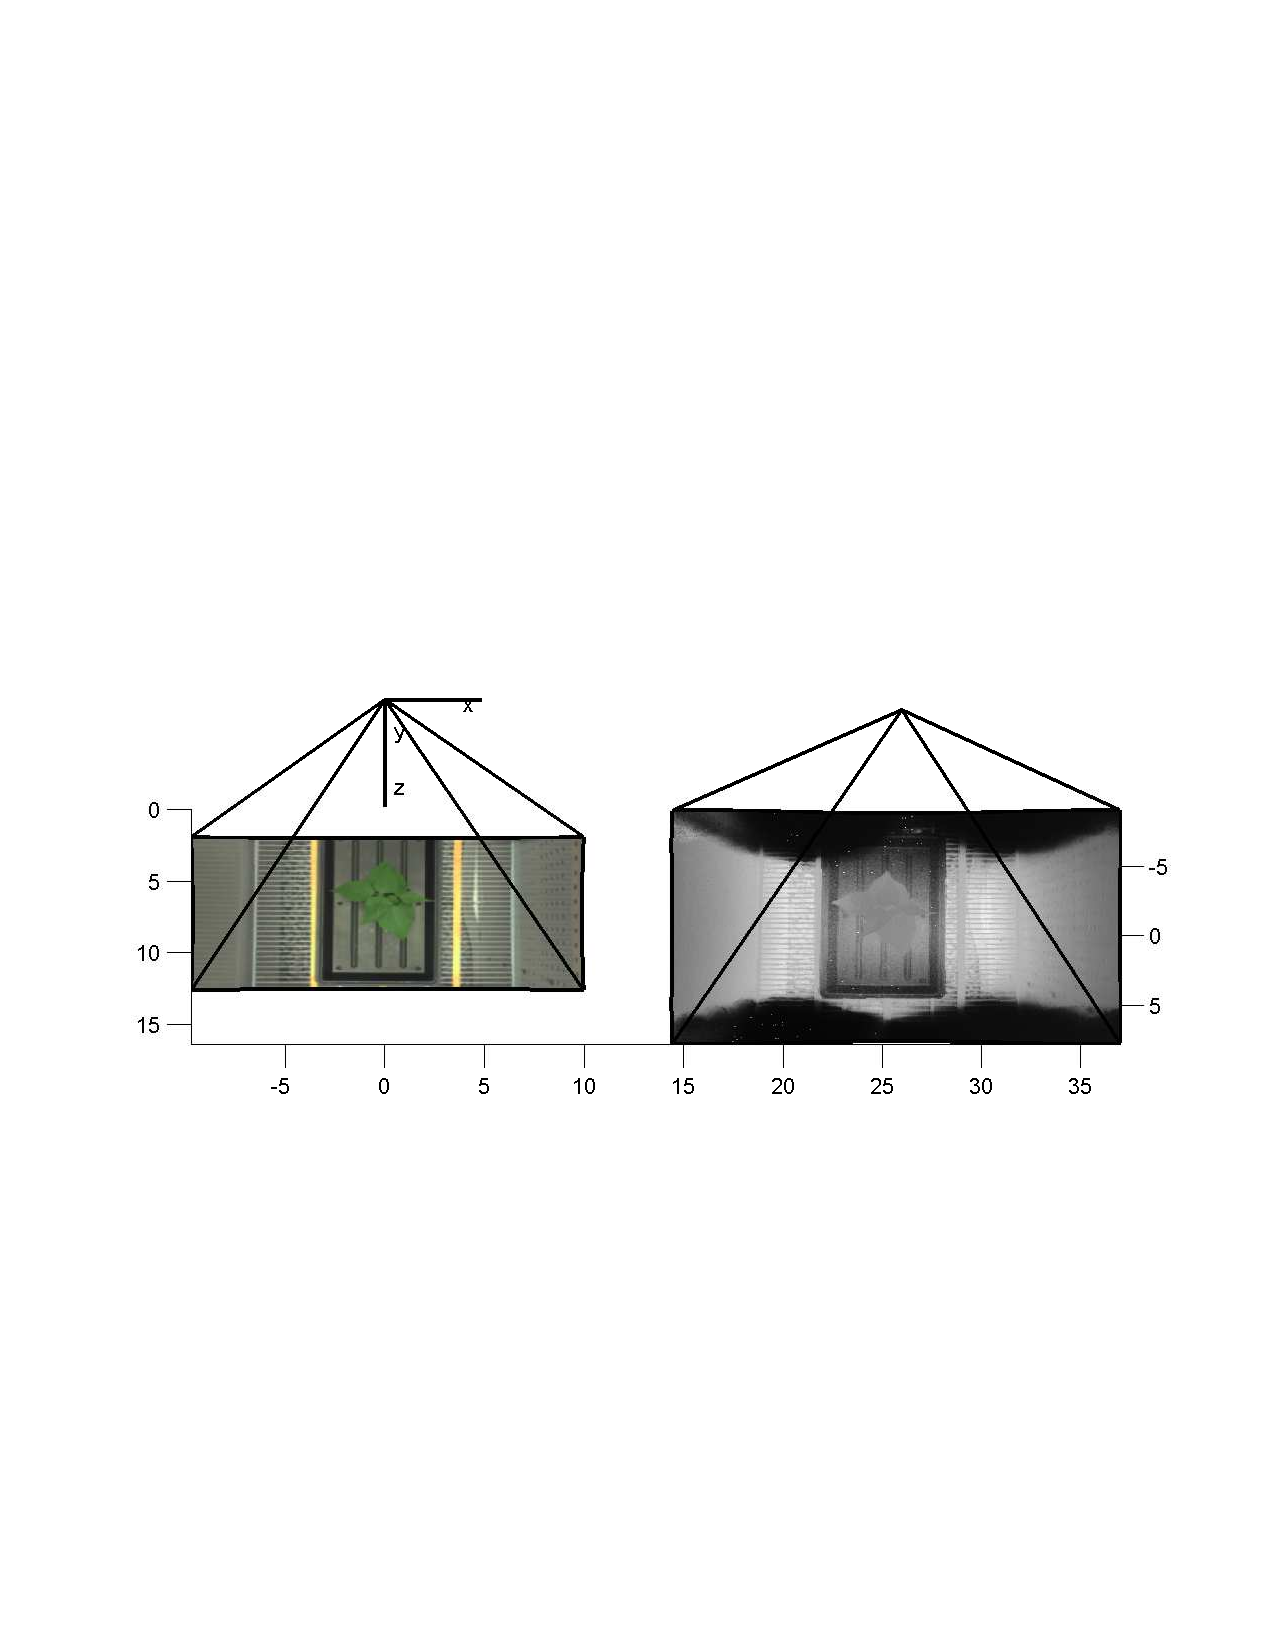
\includegraphics[width=9cm,trim=20 240 20 300,clip]{Figures/CameraConfiguration}
\caption{A plot of the three cameras showing their relative configuration and fields of view as obtained through calibration.  Units are in mm.  In the center is the color camera, and its optical center defines the world coordinate system.  On the right is the depth camera.  Its points are projected into the world coordinate system.  On the left is the fluorescent and IR camera.}
\label{fig:CameraConfiguration}
\end{figure}

\subsection{Image Accusation}

\subsection{Image Calibration}

\subsection{Creative Senz3D}

The depth and color images were collected using a Creative Senz3D sensor.  This section describes characterizes the data from this sensor, particularly the depth data.  The sensor contains both a $1280 \times 720$ color camera directed parallel to, and separated by roughly 25 mm from, a depth camera which has resolution of $320\times240$ pixels.  The depth sensor uses a flash near IR illuminator and measures the time-of-flight of the beam at each pixel to obtain dense depth estimates along with an IR reflectance at each pixel.

There are a number of limitations to the depth sensor including sources of depth error.  The primary measurement limit on the range-to-target is the strength of the reflected beam. Hence dark, matt surfaces are measured reliably only at close range on the order of 20 or 30cm.  Highly reflective surfaces also pose problems with direct reflections leading to saturation and highly unreliable depths.  In addition reflective surfaces at grazing angles are less reliably measured as little signal is reflected.  Hence in our data portions of the chamber floor visible in Fig.~\ref{fig:CameraConfiguration} are highly reflective and have incorrect depths.  Fortunately the primary goal of the depth measurements are to obtain leaf depths, and plants provide good, roughly Lambertian reflections of IR CITE{}.  Thus For these reasons the non-leaf depth pixels in the 3D data are unreliable and should be ignored.  Another limitation is that the IR illuminator is slightly offset on the left of the sensor and this results in shadows to the right of some objects, as well as mixed pixels on depth discontinuities.  Both of these can be readily detected as large standard deviations in the depth image.

\subsubsection{Sensor Calibration}

A checkerboard pattern was used to calibrate all three cameras to obtain both intrinsic and extrinsic parameters.  While the checkerboard pattern is not visible as variations in depth, it is nevertheless observed as variations in the reflected IR image whose pixels correspond to the depth pixels.  This enables the use of Zhang's method CITE{} to calculate the intrinsic parameters including a 2-parameter radial distortion of each camera, as well as a calculation of their relative poses.  The optical center of the color camera is used to define the world coordinates of our data.  The depth values of the depth camera are projected along their pixel rays and then rotated and translated by the pose of the depth camera, and thus recorded as 3D points in the world coordinate system.  Hence it is straight forward to project these points onto any of the three camera images.

\subsubsection{Depth Bias and Noise Characterization}
\label{sec:bias}

We characterized both the bias and the variance of the depth cameras as follows.  A flat printed checkerboard with a surrounding white board was positioned at a large number of poses [How many?] in front of the sensor.  The pose of the checkerboard is calculated in each case using the color and IR reflectance images.  This defines a plane relative to the depth camera which we use to calculate the ground truth depths for each pixel in the depth camera.  At each pose we collect multiple depth images; this provides both a bias and variance measurement for each pixel at multiple depths.

Next we sought to model the depth bias as a linear function of depth.  Two parameters were fit for each pixel (a linear coefficient and an offset).  The results are summarized in Fig.~\ref{fig:Bias}.  [Need more summary here.]

\begin{figure}
  %\includegraphics[]{Figures/}
\caption{Noise and Bias model}
\label{fig:Bias}
\end{figure}


In the recorded 3D data we subtracted our estimated bias, and averaged five depth images for each record.  Hence the actual depth variance for our data is $1/5$ of the the variances shown in Fig.~\ref{fig:Bias}, and the bias is zero.

Now we noticed that the chamber light shades blocked some of the depth camera field of view, and in doing so reflected some of the IR illumination.  This resulted in a bias shift of [how much?].  We removed this bias shift from the depth data.

\subsubsection{Data Description}

The data consist of 5 images per hour taken within 10 minutes of each other.  These include the fluorescent image, the IR reflectance image with the same camera, the color image, the 3D-depth and a confidence image.  The 3D-depth image is built from the depth sensor by transforming the points into world coordinates and is expressed in mm.  The confidence image is the standard deviation of the depths pixels.  This is useful for identifying pixels at depth discontinuities which are unreliably detected and result in large standard deviations.  In addition pixels with no response and saturated pixels are marked as high standard deviation. [Got to check this].


\subsection{Image Accusation}

\subsection{Image Calibration}

\section{Image Labeling}

\section{Baseline Performance}

\section{Conclusion}

\paragraph{Paragraph headings} Use paragraph headings as needed.
\begin{equation}
a^2+b^2=c^2
\end{equation}

% For one-column wide figures use
\begin{figure}
% Use the relevant command to insert your figure file.
% For example, with the graphicx package use
  
\includegraphics{example.eps}
% figure caption is below the figure
\caption{Please write your figure caption here}
\label{fig:1}       % Give a unique label
\end{figure}
%
% For two-column wide figures use
\begin{figure*}
% Use the relevant command to insert your figure file.
% For example, with the graphicx package use
  
\includegraphics[width=0.75\textwidth]{example.eps}
% figure caption is below the figure
\caption{Please write your figure caption here}
\label{fig:2}       % Give a unique label
\end{figure*}
%
% For tables use
\begin{table}
% table caption is above the table
\caption{Please write your table caption here}
\label{tab:1}       % Give a unique label
% For LaTeX tables use
\begin{tabular}{lll}
\hline\noalign{\smallskip}
first & second & third  \\
\noalign{\smallskip}\hline\noalign{\smallskip}
number & number & number \\
number & number & number \\
\noalign{\smallskip}\hline
\end{tabular}
\end{table}


%\begin{acknowledgements}
%If you'd like to thank anyone, place your comments here
%and remove the percent signs.
%\end{acknowledgements}

% BibTeX users please use one of
%\bibliographystyle{spbasic}      % basic style, author-year citations
%\bibliographystyle{spmpsci}      % mathematics and physical sciences
%\bibliographystyle{spphys}       % APS-like style for physics
%\bibliography{}   % name your BibTeX data base



{\small
\bibliographystyle{springer}
%\bibliography{/Sharefolder/Dropbox/Bibliographies/abbrev_brief,/Sharefolder/Dropbox/Bibliographies/xl-literature}
\bibliography{abbrev_brief,xl-literature}
}
\end{document}
% end of file template.tex

